% background.tex
\documentclass[main.tex]{subfiles}
\begin{document}
\chapter{Background} \label{ch:bg}
\section{Additive Manufacturing}\label{sec:AM} %Section labeling for cross-referencing
\emph{Additive Manufacturing} (AM) technologies had their beginnings in the decade of the 1980s. During this time, various independently developed patents were filed across the globe, describing a process that would construct an object by selectively adding layers of material -as opposed to removing excess matter or deforming mass to obtain a desired shape. This represents the core definition of AM: any technology where the final geometry of the manufactured object is obtained through controlled addition of material qualifies as an Additive Manufacturing technique \cite{Gibson2015}.

Advancements in the fields of computing, \emph{Computer Aided Design} (CAD), and controllers, among other technological developments, were necessary to translate the patents into working prototypes, with some eventually becoming the foundations of commercially successful companies -such as 3D Systems in 1986 and Stratasys in 1989 \cite{Gibson2015,3DSystems,Stratasys2017}. However, the basic process of AM has remained largely unchanged from its first iteration in the late 80s: First, a computer model of the object is made using CAD software and exported under the .\emph{stl} file format. Afterwards, the part geometry is stratified, or \textquotedblleft sliced\textquotedblright, and translated into machine instructions using a specialized software called \emph{slicing engine}. An AM machine then follows said instructions, commonly referred to as the \emph{toolpath}, to build the object in layers. Finally, the part is available to the user. Depending on either the requirements of the part, or the specifics of the AM technique used, some post-processing may be required \cite{Gibson2015}. A visual representation of the process is shown in Figure~\ref{fig:AM_flow}.

\begin{figure}[h]
	\center
	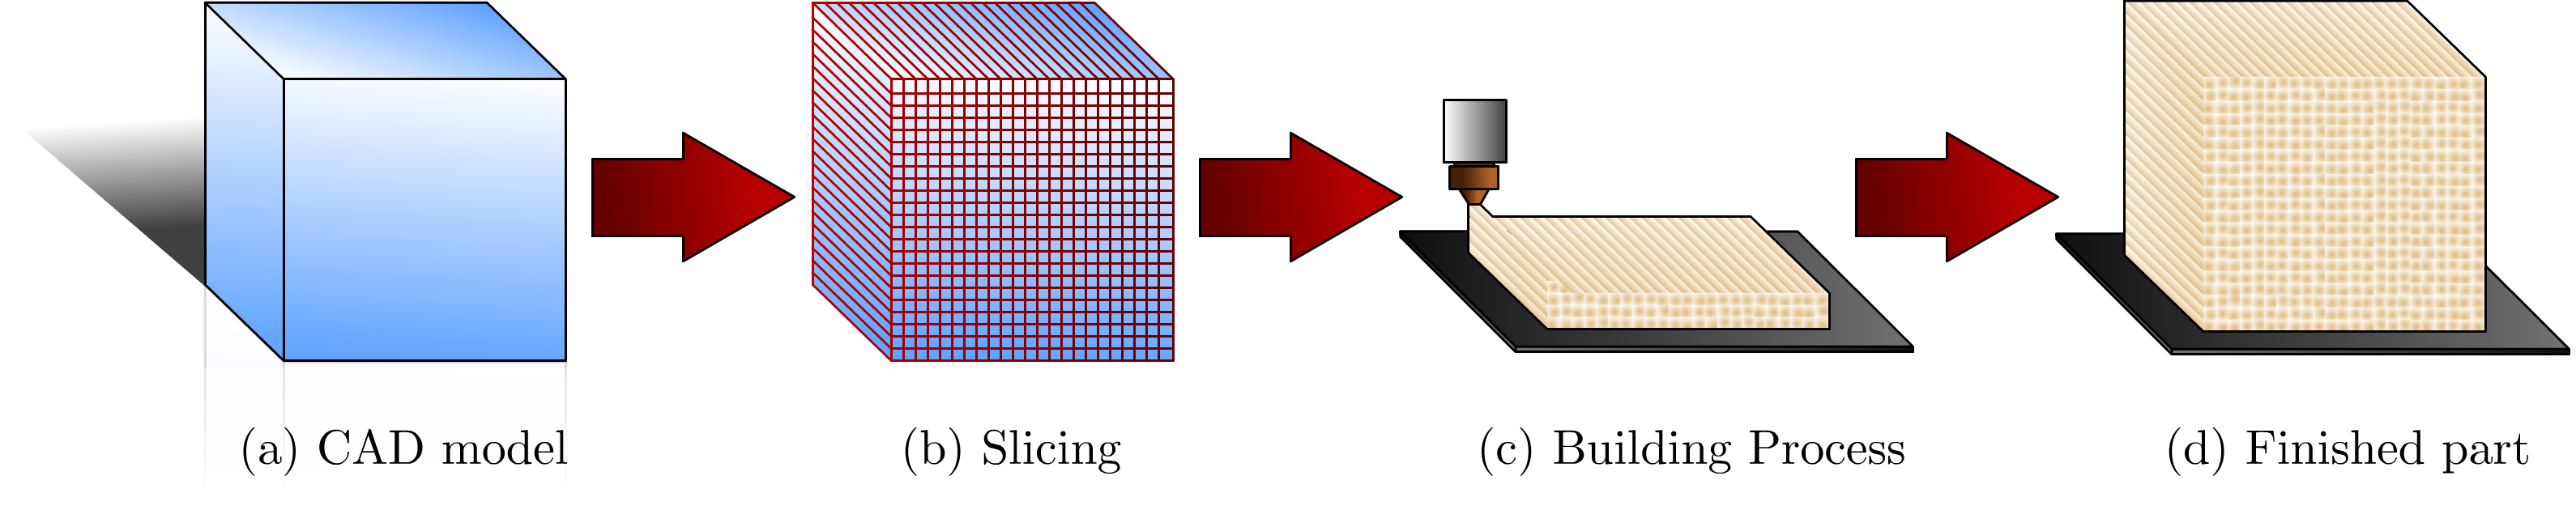
\includegraphics[width=\linewidth]{AM_flowchart_1}
	\caption{Process flow of AM} \label{fig:AM_flow}
\end{figure}
\pagebreak %Used to move the entire paragraph to a new page.
 
While all AM technologies operate on the same basic process flow described above, the specifics of each AM technique vary substantially, ranging from processes that use paper and binder, all the way through metal-based, laser tracing technologies. Since this is a rapidly evolving field, no general consensus exists for classifying the multiple AM processes available. However, the classification system proposed under the ASTM/ISO 52900 standard \cite{ASTM52900}, has been somewhat accepted by the field and divides AM technologies as follows:
\begin{enumerate}
	\item \textbf{Binder Jetting}: AM techniques where a binding agent is used to selectively promote cohesion in powder materials -generally gypsum, sand or metallic powders~\cite{ASTM52900,3DHubs2018}.
	\item \textbf{Directed Energy Deposition}: AM processes where a focused thermal energy source (i.e. laser, electron beam, plasma arc) is used to fuse materials as they are being deposited in the build volume. Materials are almost exclusively metals~\cite{ASTM52900,3DHubs2018}.
	\item \textbf{Material Extrusion}: In this type of AM technology, material is dispensed through a nozzle or orifice. Fused Filament Fabrication belongs to this classification. Materials are almost exclusively thermoplastics \cite{ASTM52900,3DHubs2018}.
	\item \textbf{Material Jetting}: AM techniques where build material is deposited selectively in droplets. Materials are usually wax or thermoplastics, but there are examples of metal-based, material jetting techniques \cite{ASTM52900,3DHubs2018}.
	\item \textbf{Powder Bed Fusion}: AM processes where portions of a powder bed are selectively fused through application of thermal energy. \emph{Selective Laser Sintering} (SLS) belongs to this category. Materials are usually thermoplastic polymers or metals \cite{ASTM52900,3DHubs2018}. 
	\item \textbf{Sheet Lamination}: In this type of AM technology, the final part is formed by bonding sheets of material -usually paper or composites \cite{ASTM52900,3DHubs2018}. 
	\item \textbf{Vat Photopolymerization}: In this AM process, a liquid photopolymer is selectively cured by a light source. \emph{Stereolithography} (SLA), arguably the first AM technology, belongs to this category. Due to the nature of this technique, the only materials used are photopolymers \cite{ASTM52900,3DHubs2018}.
\end{enumerate} 

\subsection{Advantages, Disadvantages and Success Stories}\label{subsec:AMAdDis} 
Since AM processes allow a relatively direct conversion of a CAD model into a constructed object, they were originally exclusively used for prototype development. For this reason, they were initially classified as \textquotedblleft \emph{Rapid Prototyping}\textquotedblright~(RP) technologies. This terminology is still used today, however, it is being superseded by \emph{Additive Manufacturing} since its potential to become a proper fabrication technique exists \cite{Gibson2015}. However, while being capable of quickly jumping from part design to manufacturing is a great advantage, AM has its own set of drawbacks. Table \ref{tab:AM_AdDis} summarizes the most noteworthy set of advantages and disadvantages typical of most AM technologies.

\begin{table}[h]
	\centering
	\caption{Advantages and Disadvantages of Additive Manufacturing}
	\label{tab:AM_AdDis}
	\begin{tabu} to 0.95\textwidth {  X[c]  X[c] }
		\hline
		\textbf{Advantages} & \textbf{Disadvantages} \\ 
		\hline
		Faster product development cycles \cite{Gibson2015} & Part quality highly dependent on process parameters \cite{Gibson2015}\\
		%---------
		No additional tools needed for part fabrication\cite{Gibson2015}&  Stratified build generally results in anisotropic parts \cite{Gibson2015, Capote2017}\\
		%---------
		Cost effective for small batches of parts \cite{Baumers2016,Conner2014,Berman2012}&  Costly for production of more than hundreds of parts \cite{Baumers2016,Conner2014,Berman2012}\\
		\hline
	\end{tabu}
\end{table}   

Out of all the described advantages and disadvantages, the high anisotropy of AM parts is responsible for the slow embrace of AM in highly demanding engineering fields -such as the aerospace and automotive industries. The highly anisotropic mechanical behavior makes it extremely difficult to predict part failure, therefore, it can't be implemented in engineering applications where catastrophic failure is to be avoided at all costs. Even so, success stories of implementation of AM in industrial environments are abundant. Below is a number of relatively 
recent examples:

\begin{itemize}
	\item \textbf{Volkswagen Autoeuropa}: This automotive assembly plant implemented the use of FFF machines to manufacture tools, jigs and fixtures used in their assembly line. They now produce 93\% of the tools that were historically externally sourced, and have reportedly cut their tool development time and costs by 95\% and 91\% respectively \cite{deVries2017}.
	\item \textbf{General Electric}: GE is currently producing in Alabama a complex fuel nozzle injector for the LEAP jet engine, using powder based, metal AM. The complex geometry of this component could not be manufactured by any other manufacturing technique. The production plant is expected to have 50 AM machines producing 35,000 fuel nozzle injectors annually by 2020 \cite{GEAdditive2016}. 
	\item \textbf{Adidas and New Balance}: Both shoe companies have developed separate approaches to constructing highly optimized, 3D printed midsoles for high performance running sneakers. New Balance makes use of SLS technology to build the intricate geometry of their \textquotedblleft \emph{Zante Generate}\textquotedblright~sneaker, using powdered TPU elastomer as the parent material. The designed honeycomb structure of the midsole, combined with the flexible material used, is supposed to improve the comfort and support brought by the shoe \cite{NewBalance2016}. Adidas on the other hand chose to develop the \textquotedblleft \emph{AlphaEDGE 4D LTD}\textquotedblright~running shoe using the CLIP technology by Carbon3D. While the cell geometry in  the midsole is also supposed to bring performance and comfort improvements, the final ambition of Adidas is to perfect the technology to a point where a customer can simply go to a shoe store, have their feet scanned, and receive a fully customized shoe with a 3D printed midsole that fits their particular needs \cite{Matisons2015,Saunders2018}. In both cases, the geometry of the midsole can only be produced by AM. The intricate structures in the midsoles can be seen in Figure \ref{fig:AMshoes}.
		
\end{itemize}
\begin{figure}[h]
	\center
	\subfloat[New Balance Zante Generate~\cite{NewBalance2016}\label{fig:NBZG}]{%
		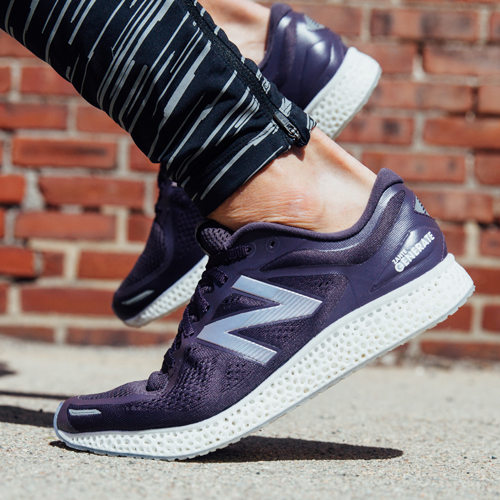
\includegraphics[height=6cm, keepaspectratio]{NB_generate}
	}
	\hfill
	\subfloat[Adidas AlphaEdge 4D LTD~\cite{Saunders2018}\label{fig:adidas}]{%
		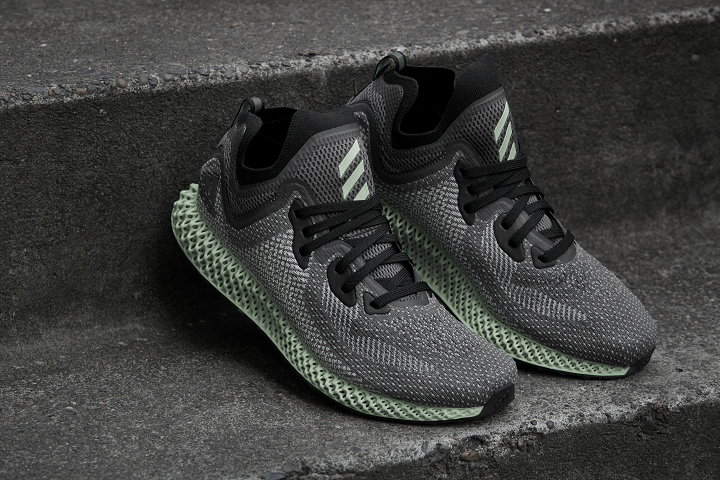
\includegraphics[height=6cm, keepaspectratio]{alphaedge_4D}
	}
	\caption{Shoes with AM midsoles}
	\label{fig:AMshoes}
\end{figure}

Note that in the cases presented, the main reason behind the usage of AM was either reduction of expenses associated with producing small batches of parts, or the capability of reproducing a unique and complex geometry. This is a trend that is observed in most of the literature describing implementation of AM into industrial scenarios.

While the advantages and disadvantages described here cover the field of AM as a whole, each technique comes with its own set of pros and cons that may make it the preferred method to reproduce a particular product or geometry. This work, however, focuses solely on FFF. The specifics of this process are described in detail in Section~\ref{sec:FFF}.

\section{Fused Filament Fabrication}\label{sec:FFF} 
\emph{Fused Filament Fabrication}~(FFF) is an AM technology where the final geometry of the part is obtained through controlled extrusion of a liquid, self-hardening material -usually a thermoplastic polymer in molten state \cite{Gibson2015}. Originally developed by Stratasys in the 1980s under the \textendash~still trademarked \textendash~\emph{Fused Deposition Modeling}~(FDM\texttrademark) moniker, it has recently become one of the most widely used AM techniques due to the advent of low-cost, desktop FFF machines in the early 2010s caused by the expiration of key patents from Stratasys \cite{Gibson2015,Capote2017}. 
\pagebreak
\subsection{The FFF process}\label{ssec:FFFmach}
At its core, the typical FFF machine consists of a heated build surface commonly referred to as a \emph{build plate}, a specialized tool known as a \emph{printhead}, and the fabrication material -supplied in the form of spools of thermoplastic polymer filament. The printhead is itself composed of a heating element, a nozzle, and some form of driving mechanism that pushes the filament downward. As the thermoplastic material is moved through the heated chamber, polymer melt is formed and extruded through the opening at the tip of the nozzle, producing a \emph{bead}. The molten polymer can then be deposited upon the build plate, where controlled movements of the printhead and the fabrication surface gradually construct the final geometry of the part in a layer-by-layer build approach~\cite{Gibson2015}. The typical setup of an FFF machine can be seen in Figure \ref{fig:machconfig}. In this example, the printhead moves in the \emph{x-y} plane, while the build plate moves in the \emph{z} direction. 
 
\begin{figure}[h]
	\center
	\subfloat[FFF printhead cross section\label{fig:FFFnoz}]{%
		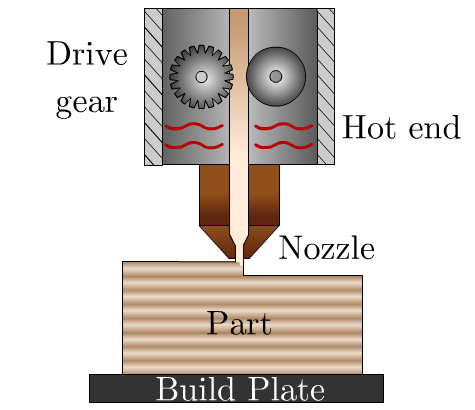
\includegraphics[height=6cm, keepaspectratio]{nozzle}
		}
	\hfill
	\subfloat[Typical FFF machine\label{fig:FFFmach}]{%
		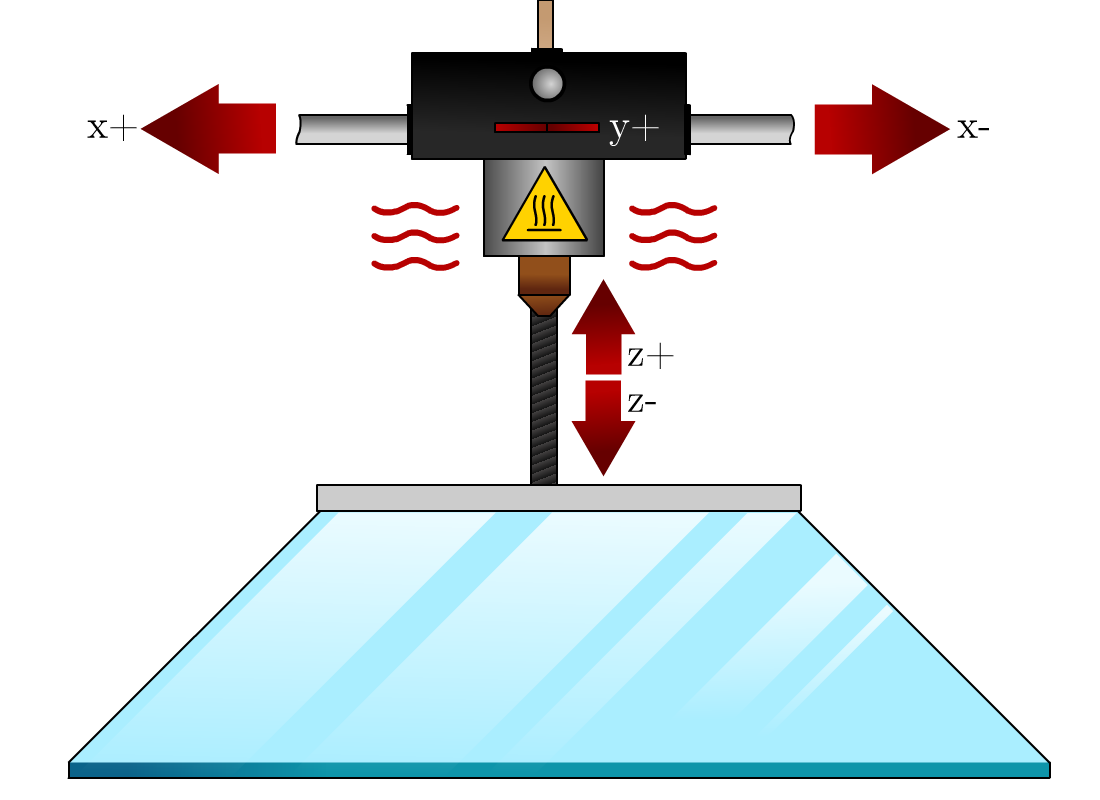
\includegraphics[height=6cm, keepaspectratio]{printer_layout}
		}
	\caption{The basic FFF machine configuration} \label{fig:machconfig}
\end{figure}
Like all AM technologies, the FFF process starts in a computer with a CAD model converted to the \emph{.stl} file format. The geometry is then translated to machine instructions through a \emph{slicing engine}, where the user inputs a plethora of process parameters that include nozzle and build plate temperatures, print speed, layer thickness and build orientation. Finally the \emph{toolpath} is executed by the FFF printer, building the object in a layer-by-layer basis \textendash~sometimes referred to as \emph{2.5D} printing~\cite{Gibson2015, VanHulle2017}. Figure \ref{fig:FFFflow} shows an abridged version of the process. The \emph{z} axis indicates the intended build direction. Note how some of the finer details in the original CAD file are lost in the printed part \textendash~due in part to the layer height and build orientation selected.

\pagebreak
\begin{figure}[h]
	\center
	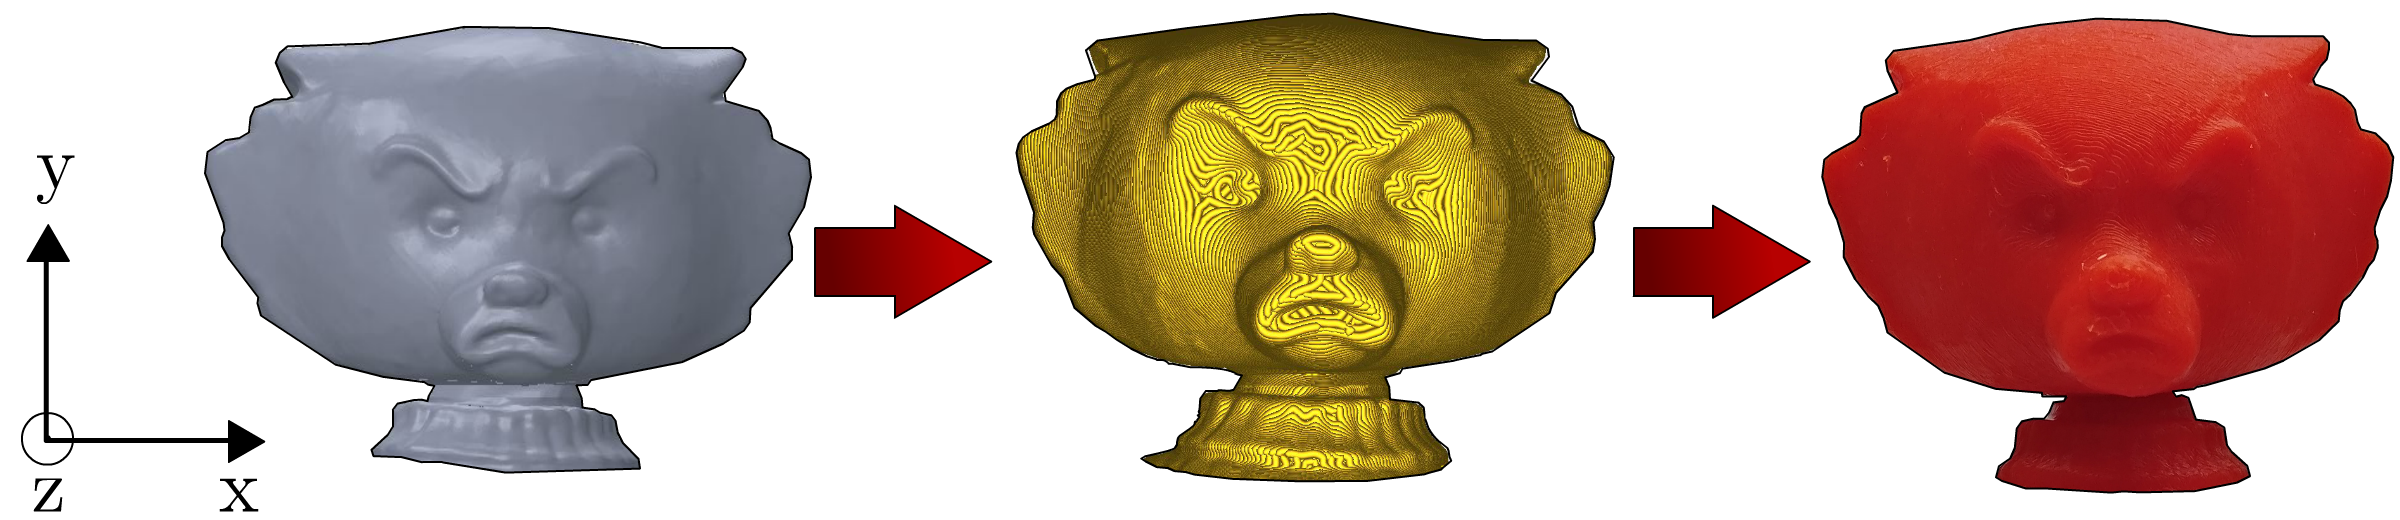
\includegraphics[width=0.95\textwidth]{FFFflow}
	\caption{From left to right: stl, toolpath and final part} \label{fig:FFFflow}
\end{figure}

The process is capable of producing complex geometries that would be otherwise hard to reproduce through other polymer processing techniques, such as injection molding. However, it is bound by the disadvantages described in Section \ref{subsec:AMAdDis}, as well its own unique set of drawbacks. Namely:

\begin{itemize}
	\item The circular orifice in the nozzle makes FFF incapable of reproducing sharp corners, limits the size of the smallest reproducible feature, and causes the final part to be filled with voids \textendash originating in the junction of round beads. These problems can be seen in Figure \ref{fig:FFFpartprob}: On the left, a comparison of a 90$^\circ$ corner planned in the toolpath and the final geometry of the printed bead is shown. Note the rounded nature of the turn. On the right, a cross section of an FFF part obtained through \emph{Micro Computer Tomography} ($\mu$CT) shows the voids that form during the printing process.
	\begin{figure}[h]
		\center
		\subfloat[FFF toolpath vs. printed bead\label{fig:FFFbead}]{%
			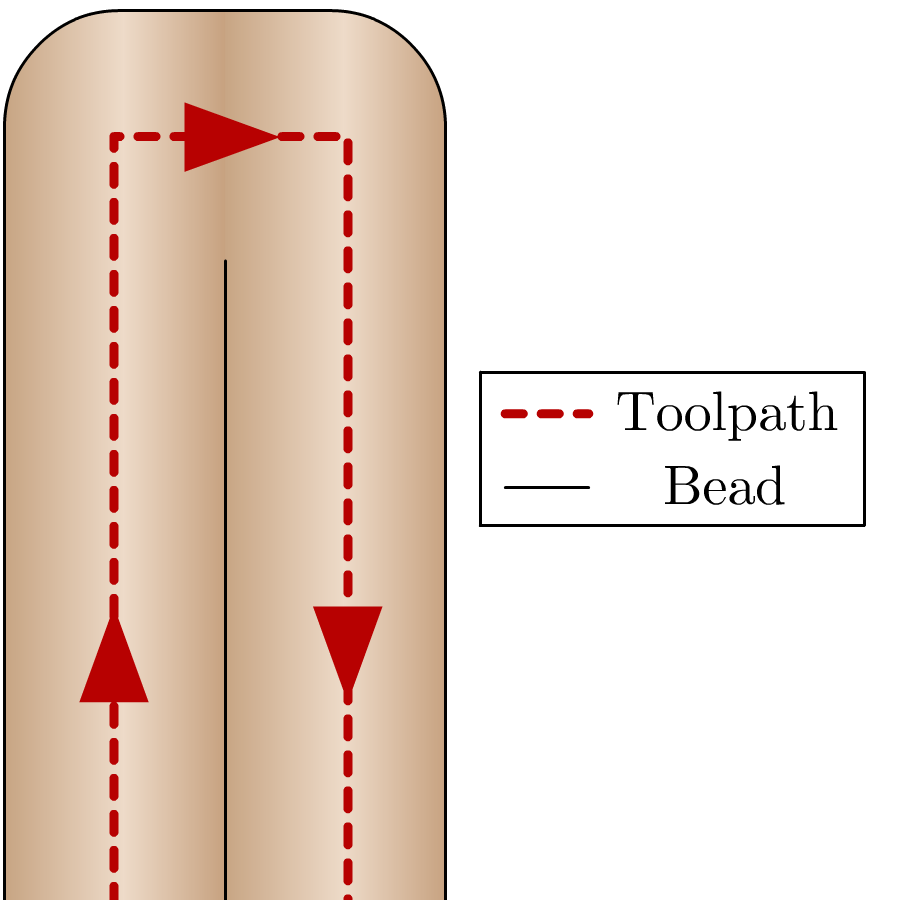
\includegraphics[height=6cm, keepaspectratio]{Toolpath}
		}
		\hfill
		\subfloat[Cross section of an FFF part\label{fig:FFFuCT}]{%
			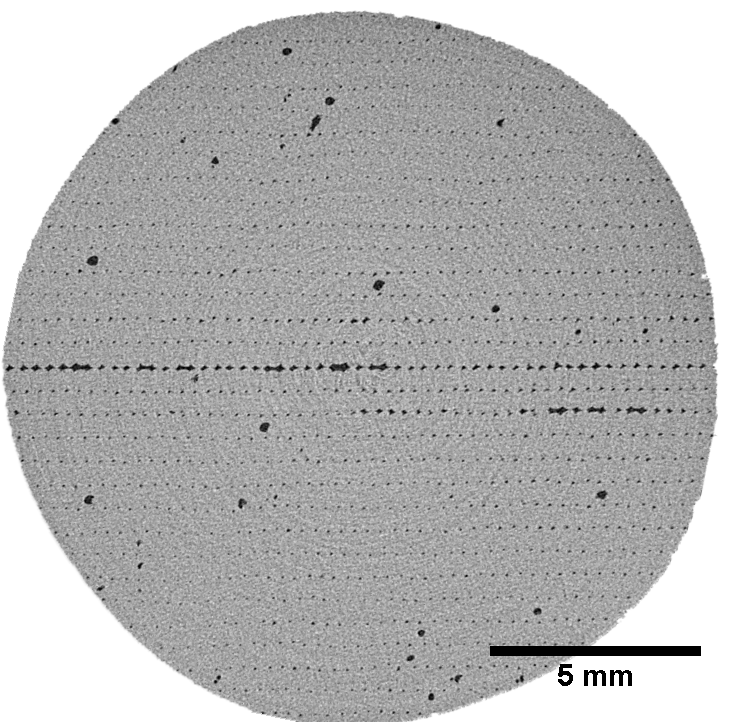
\includegraphics[height=6cm, keepaspectratio]{uCT_FFF}
		}
		\caption{Typical FFF part mesostructure and its origin} \label{fig:FFFpartprob}
	\end{figure}
	\item The junction of adjacent beads behaves akin to a polymeric weld, and has inferior mechanical properties than the bulk material \cite{Capote2017}. This, coupled with the aforementioned voids which can act as stress concentrators, causes FFF parts to behave in extremely anisotropic manner with diminished mechanical performance when compared to analogous parts obtained through traditional polymer processing technologies \textendash~such as injection molding \cite{Capote2017}.
\end{itemize}

This last disadvantage is responsible for the slow embrace of FFF as a proper manufacturing technique: the high anisotropy of FFF parts imply that predicting part failure becomes extremely difficult and thus, proper part design that guarantees safe operation of the object under important loads is hard to achieve.  For this reason, efforts to characterize the mechanical behavior of FFF parts have existed since as early as the 1990s. Recent examples are presented in Section \ref{ssec:mechPropFFF}.

\subsection{Mechanical Properties of FFF parts}\label{ssec:mechPropFFF}

Efforts have been made to characterize the mechanical anisotropy of FFF parts. However, due to the lack of testing standards and problems during toolpath planning, most studies focus solely in the tensile mechanical performance of FFF coupons.

Recent studies performed by Koch \emph{et al.} \cite{Koch2017} and Rankouhi \emph{et al.} \cite{Rankouhi2016} indicate that the final tensile properties of FFF coupons are particularly sensitive to bead orientation and proper mass output through the nozzle. Other process parameters, such as the layer thickness, have varying degrees of impact upon the final tensile strength of the part. In both studies, tensile coupons were printed with bead orientations of 0$^\circ$, 45$^\circ$ and 90$^\circ$ in the \emph{x-y} plane. Results showed that in all the experimental conditions selected, a 0$^\circ$ orientation always behaved closer to the bulk material, whereas a 90$^\circ$ sample always had significantly lower tensile strengths. The 45$^\circ$ samples sat in between both extremes. It is important to note that in both studies, toolpath manipulation was necessary to avoid premature failure of the coupons due to stress concentrators originating in void formation due to the elliptical nature of the beads. Figure \ref{fig:FFFmechProp} shows some of the results by Koch \emph{et al}. The geometry corresponds to an ASTM Type I Tensile coupon. Injection molded results are denoted \emph{IM} for comparison. Note that the 90$^\circ$ orientation had a tensile strength that was 25\% inferior to the IM counterpart, and 20\% worse than the 0$^\circ$ oriented FFF coupon. This is a prevalent trend in the consulted bibliography.

Literature for other types of mechanical testing of FFF parts is relatively scarce when compared to tension experiments. Research indicates that the compressive strength of FFF parts tends to be higher than the tensile strength, as well as being less sensitive to process parameters \textemdash the bead orientation in particular seems to have a significantly diminished impact upon the compressive strength when compared to its effect upon tensile tests \cite{Ahn2002,Lee2007}. Shear strength results are virtually non-existent.

\pagebreak
\begin{figure}[h]
	\center
	\subfloat[Tensile strength of tensile coupons\label{fig:KochCoup}]{%
		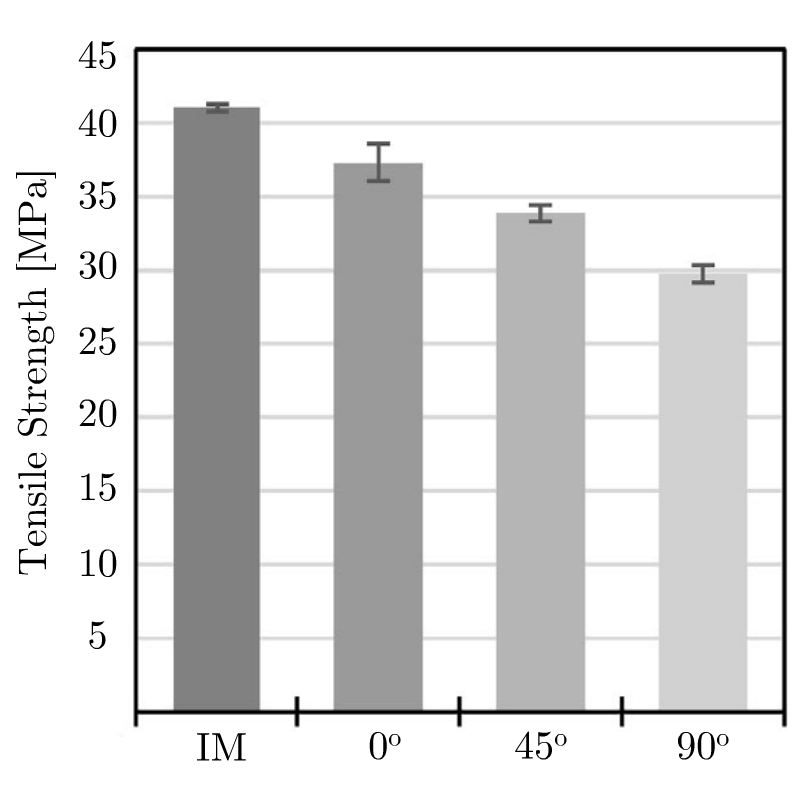
\includegraphics[height=6cm, keepaspectratio]{lit_mechpropFFF}
	}
	\hfill
	\subfloat[Representation of coupons used\label{fig:KochRes}]{%
		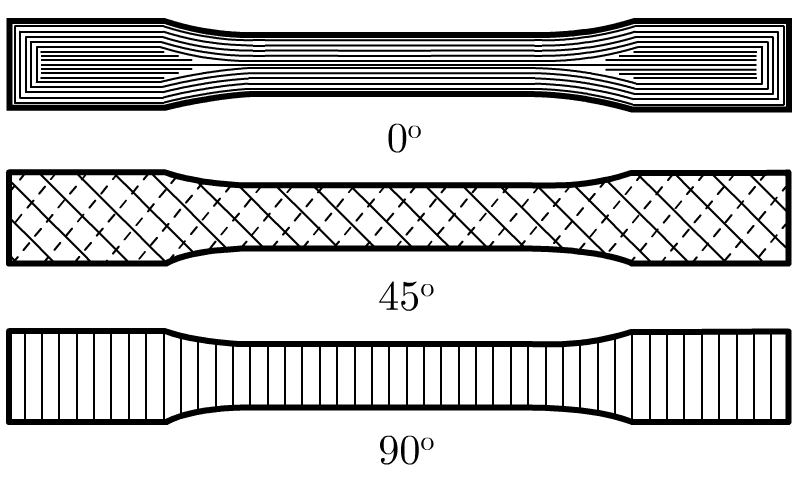
\includegraphics[height=4cm, keepaspectratio]{lit_mechpropFFF2}
	}
	\caption{Results from Koch \emph{et al.} \cite{Koch2017}} \label{fig:FFFmechProp}
\end{figure}

\section{Failure Criteria}\label{sec:FC}   
The increased use of advanced materials in industry has brought upon a necessity to properly characterize their strengths and failure modes. Composites in particular are commonly used in highly demanding engineering fields given that they excel in mechanical properties. However, due to their very nature, their behavior is extremely anisotropic. For this reason, it has been of great interest to develop a proper way to model the behavior of anisotropic materials under mechanical stresses as a way to predict part failure \textendash~a practice from here on referred to as developing a \emph{failure criterion}. 

Early attempts to properly predict failure of anisotropic materials go as far back as 1948 with the Hill model \cite{Osswald2017a}. Further developments led to a plethora of failure criteria, such as the Tsai-Hill, Malmeister, Tsai-Wu, Gol'denblat-Kopnov, Puck, and Cuntze to name a few \cite{Osswald2017a,Osswald2015}. A wide variety of criteria exists because a model will rarely capture the complete failure behavior of an anisotropic material. To illustrate this point, refer to Figure \ref{fig:FCComp}, reproduced from work by Sun \emph{et al}. \cite{Sun1996} where a composite Glass fiber-Epoxy laminate was loaded biaxially, in a direction that was either parallel ($\sigma_{11}$), perpendicular ($\sigma_{22}$) to the fiber, or a combination of both. Positive stresses indicate tensile load, while negative values point to compressive forces. The data, represented by the white squares, does not agree with any of the used models in the fourth quadrant of the graph. This type of behavior is common throughout the literature: Puck's model is great at predicting shear strengthening effects, but doesn't perform well when dealing with combined axial loading scenarios; the Gol'denblat-Kopnov model by contrast is great at predicting axial stress interactions, but falls short when dealing with shear strengthening effects caused by combined shear-axial loadings. These trends point to the limitations of each model: in order to either facilitate calculations, or due to the difficulty of performing combined loading tests, interaction effects are neglected either by mathematical choice, or indirectly through the inner workings of the failure criterion \cite{Osswald2017a}.  

\begin{figure}[h]
	\center
	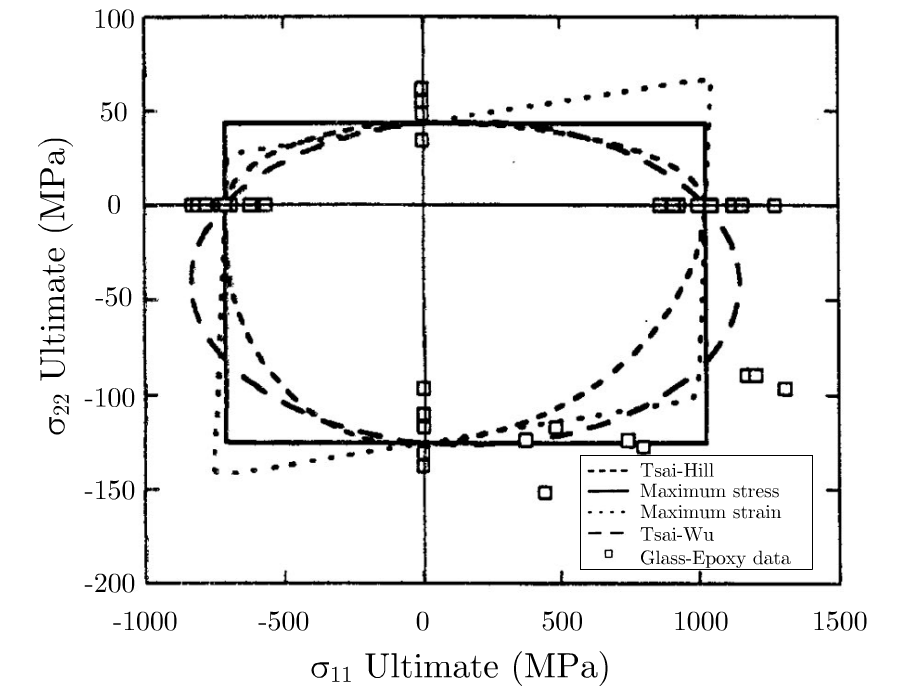
\includegraphics[height=10cm, keepaspectratio]{FC_comparison}
	\caption{Comparison of different Failure criteria. \cite{Sun1996}} \label{fig:FCComp}
\end{figure}     

Properly mapping a failure surface through a criterion proves to be an invaluable tool for design, since it allows engineers to assess if a part will perform safely under its intended loading conditions. Such tool could in theory help overcome the main shortcoming of FFF since a properly tailored failure envelope would allow proper part design considerations. However, since no present criterion completely captures the behavior of anisotropic materials, a novel technique is needed. Chapter \ref{ch:oocrit} describes in detail a novel approach, based on the Gol'denblat-Kopnov model, that includes interaction effects to properly describe the failure behavior of anisotropic parts.
% Nomenclature introduced in this chapter:
\nomenclature[A]{SLA}{Stereolithography}% 
\nomenclature[A]{SLS}{Selective Laser Sintering}%
\nomenclature[A]{$\mu$CT}{Micro Computer Tomography}%

% Symbols introduced in this chapter:
\nomenclature[S]{$\sigma$}{Axial stress \nomunit{$MPa$}}
\nomenclature[S]{$\tau$}{Shear stress \nomunit{$MPa$}}
\nomenclature[S]{$\sigma_{11}$}{Axial stress in the 1-1 direction \nomunit{$MPa$}}
\nomenclature[S]{$\sigma_{22}$}{Axial stress in the 2-2 direction \nomunit{$MPa$}}
\nomenclature[S]{$\sigma_{33}$}{Axial stress in the 3-3 direction \nomunit{$MPa$}}
\nomenclature[S]{$\tau_{12}$}{Shear stress in the 1-2 plane \nomunit{$MPa$}}
\nomenclature[S]{$\tau_{13}$}{Shear stress in the 1-3 plane \nomunit{$MPa$}}
\nomenclature[S]{$\tau_{23}$}{Shear stress in the 2-3 plane \nomunit{$MPa$}}
\end{document}